%%%%%%%%%%%%%%%%%%%%%%%%%%%%%%%%%%%%%%%%%%%%%%%%%%%%%%%%%%%%%%%%
% This intro/reminder comes after a first course on sequence
% processing with 1D NNet for discrete sequence. 
% reminder: sequence of discrete symbols
% - examples of application
% - + exemples of Human activity / audio classification
% - embeddings
% - COnv 1D
% - Pooling

% Alphabet = set of nucleotides: 
% A,C,G,T
\newcommand{\cga}{{\color{red!70!black} A}}
\newcommand{\cgc}{{\color{blue!70!black} C}}
\newcommand{\cgg}{{\color{yellow!70!black} G}}
\newcommand{\cgt}{{\color{green!70!black} T}}

\begin{frame}{Sequence of discrete symbols classification }
  \begin{block}{Movie review classification}
    \begin{center}
      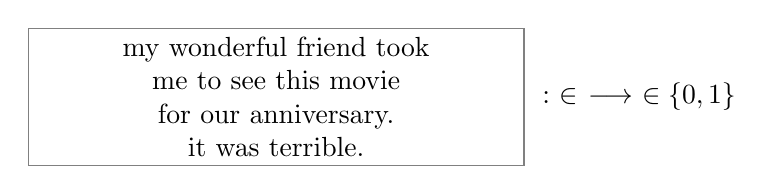
\begin{tikzpicture}
        %%%%%%%%%%%%%%%%%%%%% 
        \node[anchor=east,draw=gray,text width=0.5\textwidth,align=center] (review) at
        (0,0) {my wonderful friend took me to see this movie \\for our
          anniversary. \\ it was terrible.};
        %%%%%%%%%%%%%%%%%%%%% 
        \node[anchor=west] (txt) at (0.1,0) {$: \ \x \in \real^{\nfeats} \ \longrightarrow \ \class \in\{0, 1\}$};
      \end{tikzpicture}
    \end{center}
  \end{block}
  \begin{block}{Enhancer Identification in  DNA Sequences}
    \begin{center}
      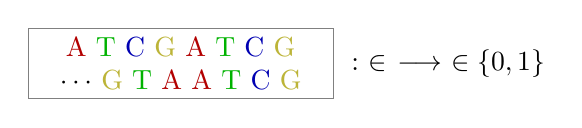
\begin{tikzpicture}
        %%%%%%%%%%%%%%%%%%%%% 
        \node[anchor=east,draw=gray,text width=0.3\textwidth,align=center] (review) at
        (0,0) {\cga~\cgt~\cgc~\cgg~\cga~\cgt~\cgc~\cgg\\$\cdots$~\cgg~\cgt~\cga~\cga~\cgt~\cgc~\cgg};
        %%%%%%%%%%%%%%%%%%%%% 
        \node[anchor=west] (txt) at (0.1,0) {$: \ \x \in \real^{\nfeats} \ \longrightarrow \ \class \in\{0, 1\}$};
      \end{tikzpicture}
    \end{center}
  \end{block}
  \begin{itemize}
  \item $\dataset= (\exi , \classi )_{i=1}^{\nsamples}$ 
  \item The input is a sequence $\rightarrow$ how to build $\x$ ? 
  \item A sequence of discrete symbols $\in \vocab$
  \item Symbols  interact with each other, the neighborhood is important
  \end{itemize}
\end{frame}


%%%%%%%%%%%%%%%%%%%%%%%%%%%%%%%%%%%%%%%%%%%%%%%%%%%%%%%%%%%%%%%%%%
\begin{frame}{Embedding of discrete symbols}
    \begin{center}
      \begin{displaymath}
          \begin{array}{lcccccccc}
            \seq{s}=&[ &\cgc&\cga&\cgt&\cgt&\cgg&\cgt
                        &]\\
            &&\downarrow &\downarrow &\downarrow &\downarrow &\downarrow &\downarrow \\
            \textrm{Look-up}&&\wemb &\wemb &\wemb &\wemb &\wemb &\wemb  \\
               &&\wvector_{\cgc}&\wvector_{\cga}&\wvector_{\cgt}&\wvector_{\cgt}&\wvector_{\cgg}&\wvector_{\cgt} \\
          \end{array}
        \end{displaymath}
        {\huge $\downarrow$} \\
        \tikz{\draw[step=0.5,black,thin] (0,0) grid (3,2);}
    \end{center}
\end{frame}

%%%%%%%%%%%%%%%%%%%%%%%%%%%%%%%%%%%%%%%%%%%%%%%%%%%%%%%%%%%%%%%%%%
% In pytorch the indices are :
% batch, channel, data-point
% The data point for a 1D input is (t,d)
% For an image it is (x,y)
\begin{frame}{Convolution 1D}
  \framesubtitle{Extract a frame, or a window, and apply a ``filter''}
  \begin{columns}
    \column{0.6\textwidth}
    %%% the input : a matrix + window
    \begin{center}
    The input sequence of  $L=6$ \\vectors in $\real^{\nfeats}$,  $\nfeats=4$ \\[1ex]
    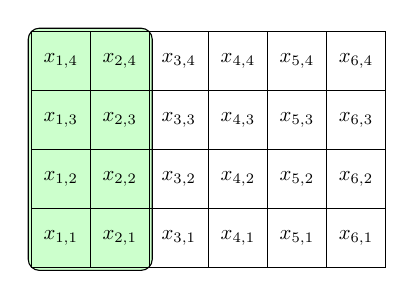
\begin{tikzpicture}[scale=0.75,every node/.style={scale=0.75}]
      % the window
      % offset for x and y of .5 + a bit more 
      \draw[fill=green!20,rounded corners] (0.45,0.45) rectangle (2.55,4.55); % green 
      %% the grid 
      \foreach \l in {1,2,...,4}
      \foreach \c in {1,2,...,6}
      {
        \draw (\c,\l) +(-.5,-.5) rectangle ++(.5,.5);
        \draw (\c,\l) node{$x_{\c,\l}$};
      }
    \end{tikzpicture}
  \end{center}
    \column{0.6\textwidth}
    \begin{center}
    The filter:\\kernel size of $ks=2$\\[1ex]
    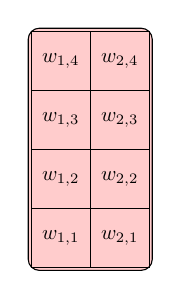
\begin{tikzpicture}[scale=0.75,every node/.style={scale=0.75}]
      % the window
      % offset for x and y of .5 + a bit more 
      \draw[fill=red!20,rounded corners] (0.45,0.45) rectangle (2.55,4.55); % green 
      
      %% the grid 
      \foreach \l in {1,2,...,4}
      \foreach \c in {1,2}
      {
        \draw (\c,\l) +(-.5,-.5) rectangle ++(.5,.5);
        \draw (\c,\l) node{$w_{\c,\l}$};
      }
    \end{tikzpicture}
  \end{center}
\end{columns}
\begin{block}{The output value (output channel)}
  $$
  \textrm{At time }t = 1,\ {\color{red!70!black} h_1} = \sum_{i,j} {\color{red!70!black}w_{i,j}}\times  {\color{green!70!black}x_{i,j}}
  $$
\end{block}
\end{frame}



%%%%%%%%%%%%%%%%%%%%%%%%%%%%%%%%%%%%%%%%%%%%%%%%%%%%%%%%%%%%%%%%%%%%%%%%%%%
\newcommand{\xs}{4}
\newcommand{\ys}{-4}
\begin{frame}{Convolution 1D}
  \framesubtitle{Stride, or a sliding window}
  The input  is a matrix $(L=6,d=4)$, one filter of kernel size $=2$:~\\[1ex]
  \begin{block}{With a stride $= 1$}
    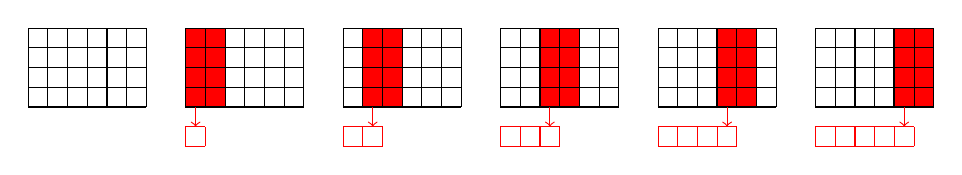
\begin{tikzpicture}[scale=0.5]
      %% the grid 
      \draw[step=0.5,black,thin] (0,0) grid (3,2);
      %%%%%%% 1 
      \draw[fill=red] (0+\xs,0) rectangle (1+\xs,2); % red 
      \draw[step=0.5,black,thin] (0+\xs,0) grid (3+\xs,2); % grid
      \draw[step=0.5,red] (-0.01+\xs,-0.5) grid (0.5+\xs,-1);    % grid res
      % arrow
      \draw[->,red]   (0.25+\xs,0) --  (0.25+\xs,-0.5);
      %%%%%%% 2 
      \draw[fill=red] (0.5+2*\xs,0) rectangle (1.5+2*\xs,2); % red 
      \draw[step=0.5,black,thin] (-0.01+2*\xs,0) grid (3+2*\xs,2); % grid
      \draw[step=0.5,red] (-0.01+2*\xs,-0.5) grid (1+2*\xs,-1);    % grid res
      % arrow
      \draw[->,red]   (0.75+2*\xs,0) --  (0.75+2*\xs,-0.5);

      %%%%%%% 3 
      \draw[fill=red] (0.99+3*\xs,0) rectangle (2+3*\xs,2); % red 
      \draw[step=0.5,black,thin] (-0.01+3*\xs,0) grid (3+3*\xs,2); % grid
      \draw[step=0.5,red] (-0.01+3*\xs,-0.5) grid (1.5+3*\xs,-1);    % grid res
      % arrow
      \draw[->,red]   (1.25+3*\xs,0) --  (1.25+3*\xs,-0.5);

      %%%%%%% 4
      \draw[fill=red] (1.49+4*\xs,0) rectangle (2.5+4*\xs,2); % red 
      \draw[step=0.5,black,thin] (-0.01+4*\xs,0) grid (3+4*\xs,2); % grid
      \draw[step=0.5,red] (-0.01+4*\xs,-0.5) grid (2+4*\xs,-1);    % grid res
      % arrow
      \draw[->,red]   (1.75+4*\xs,0) --  (1.75+4*\xs,-0.5);

      %%%%%%% 5 
      \draw[fill=red] (1.99+5*\xs,0) rectangle (3+5*\xs,2); % red 
      \draw[step=0.5,black,thin] (-0.01+5*\xs,0) grid (3+5*\xs,2); % grid
      \draw[step=0.5,red] (-0.01+5*\xs,-0.5) grid (2.5+5*\xs,-1);    % grid res
      % arrow
      \draw[->,red]   (2.25+5*\xs,0) --  (2.25+5*\xs,-0.5);
    \end{tikzpicture}
  \end{block}
  \begin{block}{With a stride = 2}
    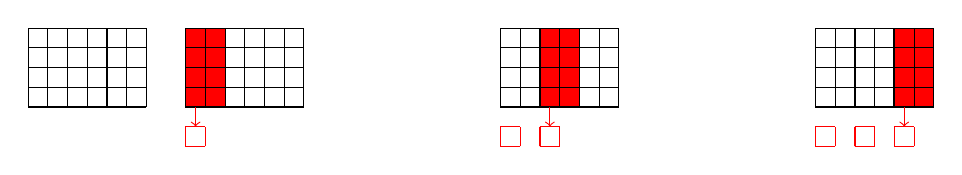
\begin{tikzpicture}[scale=0.5]
      %% the grid 
      \draw[step=0.5,black,thin] (0,0) grid (3,2);
      %%%%%%% 1 
      \draw[fill=red] (0+\xs,0) rectangle (1+\xs,2); % red 
      \draw[step=0.5,black,thin] (0+\xs,0) grid (3+\xs,2); % grid
      \draw[step=0.5,red] (-0.01+\xs,-0.5) grid (0.5+\xs,-1);    % grid res
      \draw[->,red]   (0.25+\xs,0) --  (0.25+\xs,-0.5);       % arrow

      %%%%%%% 3 
      \draw[fill=red] (0.99+3*\xs,0) rectangle (2+3*\xs,2); % red 
      \draw[step=0.5,black,thin] (-0.01+3*\xs,0) grid (3+3*\xs,2); % grid
      \draw[step=0.5,red] (-0.01+3*\xs,-0.5) grid (0.5+3*\xs,-1);    % grid res
      \draw[step=0.5,red] (-0.01+3*\xs+1,-0.5) grid (1.5+3*\xs,-1);    % grid res
      % arrow
      \draw[->,red]   (1.25+3*\xs,0) --  (1.25+3*\xs,-0.5);
      %%%%%%% 5 
      \draw[fill=red] (1.99+5*\xs,0) rectangle (3+5*\xs,2); % red 
      \draw[step=0.5,black,thin] (-0.01+5*\xs,0) grid (3+5*\xs,2); % grid
      \draw[step=0.5,red] (-0.01+5*\xs,-0.5) grid (0.5+5*\xs,-1);    % grid res
      \draw[step=0.5,red] (-0.01+5*\xs+1,-0.5) grid (1.5+5*\xs,-1);    % grid res
      \draw[step=0.5,red] (-0.01+5*\xs+2,-0.5) grid (2.5+5*\xs,-1);    % grid res
      % arrow
      \draw[->,red]   (2.25+5*\xs,0) --  (2.25+5*\xs,-0.5);
    \end{tikzpicture}
  \end{block}
\end{frame}


%%%%%%%%%%%%%%%%%%%%%%%%%%%%%%%%%%%%%%%%%%%%%%%%%%%%%%%%%%%%%%%%%%%%%%%%%%%%%%%%%%%%%%%% 
\begin{frame}{Convolution 1D}
  \framesubtitle{With 2 output channels}
  \begin{columns}
    \column{0.6\textwidth}
    %%% the input : a matrix + window
    \begin{center}
      $L=6$,  $\nfeats=4$ \\[1ex]
      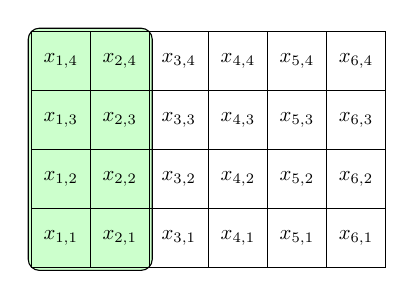
\begin{tikzpicture}[scale=0.75,every node/.style={scale=0.75}]
        % the window
        % offset for x and y of .5 + a bit more 
        \draw[fill=green!20,rounded corners] (0.45,0.45) rectangle (2.55,4.55); % green 
        %% the grid 
        \foreach \l in {1,2,...,4}
        \foreach \c in {1,2,...,6}
        {
          \draw (\c,\l) +(-.5,-.5) rectangle ++(.5,.5);
          \draw (\c,\l) node{$x_{\c,\l}$};
        }
      \end{tikzpicture}
    \end{center}
    \column{0.4\textwidth}
    \begin{center}
      Filters:kernel size of $ks=2$\\[1ex]
      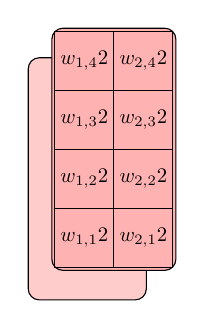
\begin{tikzpicture}[scale=0.75,every node/.style={scale=0.75}]
        % the window
        % offset for x and y of .5 + a bit more 
        \draw[fill=red!20,rounded corners] (0.05,-0.05) rectangle (2.05,4.05); % first 
        \draw[fill=red!30,rounded corners] (0.45,0.45) rectangle (2.55,4.55); 
        %% the grid 
        \foreach \l in {1,2,...,4}
        \foreach \c in {1,2}
        {
          \draw (\c,\l) +(-.5,-.5) rectangle ++(.5,.5);
          \draw (\c,\l) node{$w_{\c,\l}\lid{2}$};
        }
      \end{tikzpicture}
    \end{center}
  \end{columns}
  \begin{block}{The output value (output channel)}
    \begin{align*}
      {\color{red!70!black} h_{1,1}} &= \sum_{i,j} {\color{red!70!black}w_{i,j}\lid{1}}\times  {\color{green!70!black}x_{i,j}} \\
      {\color{red!70!black} h_{2,1}} &= \sum_{i,j} {\color{red!70!black}w_{i,j}\lid{2}}\times  {\color{green!70!black}x_{i,j}} 
    \end{align*}
  \end{block}
\end{frame}


%%%%%%%%%%%%%%%%%%%%%%%%%%%%%%%%%%%%%%%%%%%%%%%%%%%%%%%%%%%%%%%%%%%%%%%%%%%%%%%%%%%%%%%% 
\begin{frame}{Another wiew for two output channels}
  \begin{columns}
    \column{0.5\textwidth}
    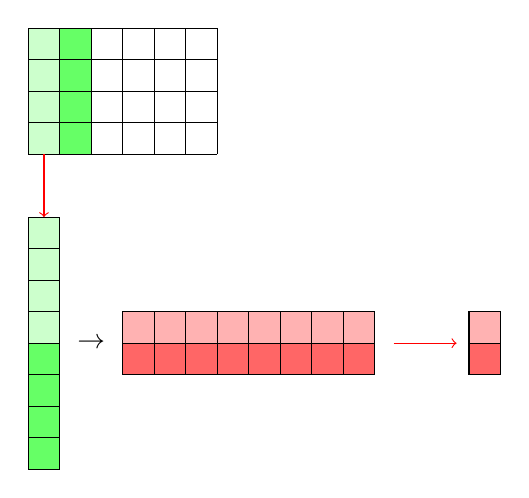
\begin{tikzpicture}[scale=0.8]
      %%%%%%% the sentence as a matrix
    \draw[fill=green!20] (0,0) rectangle (0.5,2); % red 
    \draw[fill=green!60] (0.5,0) rectangle (1,2); % red 
    \draw[step=0.5,black,thin] (0,0) grid (3,2); % grid
    %%%%% window extract 
    \draw[fill=green!60] (0,-1+\ys) rectangle (0.5,1+\ys); % red
    \draw[fill=green!20] (0,1+\ys) rectangle (0.5,3+\ys); % red
    \draw[step=0.5,black,thin] (0,-1+\ys) grid (0.5,3+\ys); % grid
    %%%  
    \draw[->,red] (0.25,0) -- (0.25,-1); % arrow
    %%% Filter 
    \node (times) at (1,1+\ys) {$\rightarrow$};
    \draw[fill=red!60] (1.49,0.5+\ys) rectangle (1.5+4,1+\ys); % colors
    \draw[fill=red!30] (1.49,1+\ys) rectangle (1.5+4,1.5+\ys); % colors 
    \draw[step=0.5,black] (1.49,0.5+\ys) grid (1.5+4,1.5+\ys); % grid
    \node (times) at (4,-0.5+\ys) {$\W$};
    %%%
    \draw[->,red] (5.8,1+\ys) -- (6.8,1+\ys); % arrow
    \draw[fill=red!60] (7-0.01,0.5+\ys) rectangle (7.5,1+\ys); % grid
    \draw[fill=red!30] (7-0.01,1+\ys) rectangle (7.5,1.5+\ys); % grid
    \draw[step=0.5,thin] (7-0.01,0.5+\ys) grid (7.5,1.5+\ys); % grid
  \end{tikzpicture}
  \column{0.5\textwidth}
  \begin{itemize}
  \item {\color{red!30!black} Two filters } applied to the same {\color{green!30!black} frame (or window)}
  \item Each filter generates one feature 
  \item[$\rightarrow$]  a vector of two values, two features $( h_{1,1},  h_{2,1})$
  \item $ h_{c,t}$ is the feature extracted for the channel $c$ at time $t$. 
  \item $\W$ gathers the parameters of the filters in one matrix
  \item The parameters $\W$ are learnt
  \end{itemize}
\end{columns}

\end{frame}

%%%%%%%%%%%%%%%%%%%%%%%%%%%%%%%%%%%%%%%%%%%%%%%%%%%%%%%%%%%%%%%%%%%%%%%%%%%%%%%%%%%%%%%% 
\begin{frame}{Exercise}
  \begin{block}{Stride}
    \begin{itemize}
    \item With an input of length $L$, a kernel size of $ks$ and a stride $=1$, what is the output dimension ?
      %% L-ks + 1 
    \item And with a stride $=2$, what is the output dimension ?
      %% (L-ks)/2 + 1
    \item With a stride of $s$ ? 
    \end{itemize}
  \end{block}
  \begin{block}{Side effect}
    \begin{itemize}
    \item The first (and last) time steps are not processed as the others. How to correct this aspects ?
    \item How to ensure the same length in output (assuming a stride of 1)  ?
      % half padding 
    \item How to ensure that every  inputs are ``seen'' equally ?
      % full padding
    \end{itemize}
  \end{block}
\end{frame}


\begin{frame}{Pooling over time}
    \begin{center}
    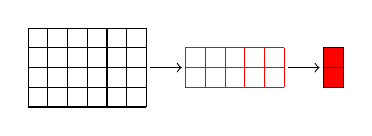
\begin{tikzpicture}[scale=0.5]
      %% the grid
      \draw[step=0.5,black,thin] (0,0) grid (3,2);
      \draw[->] (3.1,1)-- (3.9,1);
      \draw[step=0.5,red,thin] (3.99,0.5) grid (6.5,1.5);
      \draw[->] (6.6,1)-- (7.4,1);
      
      %%%%%%% final
      \draw[fill=red] (7.5,0.5) rectangle  (8,1.5); 
      \draw[step=0.5,black] (7.5,0.5) grid (8,1.5); % grid res
    \end{tikzpicture}
  \end{center}
  \begin{itemize}
  \item Mean pooling
  \item Max pooling, and $k$-max pooling
  \end{itemize}
\end{frame}

\begin{frame}{Exercise}
  % 1/ input x: 
  % 2/ conv filter -> h1, h2
  % 3/ pooling -> o

  \begin{columns}
    %%%%%%%%% 1st column the figs
    \column{0.34\textwidth}
    \begin{center}
      %%%%%% the filter 
      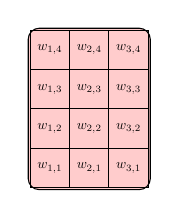
\begin{tikzpicture}[scale=0.5,every node/.style={scale=0.5}]
        % the window
        % offset for x and y of .5 + a bit more 
        \draw[fill=red!20,rounded corners] (0.45,0.45) rectangle (3.55,4.55); % green 
        
        %% the grid 
        \foreach \l in {1,2,...,4}
        \foreach \c in {1,2,3}
        {
          \draw (\c,\l) +(-.5,-.5) rectangle ++(.5,.5);
          \draw (\c,\l) node{$w_{\c,\l}$};
        }
      \end{tikzpicture}\\
      %%% First application 
      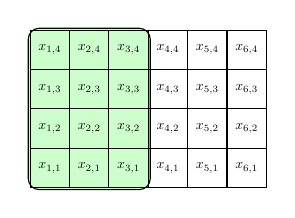
\begin{tikzpicture}[scale=0.5,every node/.style={scale=0.5}]
        % the window
        % offset for x and y of .5 + a bit more (or less)
        \draw[fill=green!20,rounded corners] (0.45,0.45) rectangle (3.55,4.55); % green 
        %% the grid 
        \foreach \l in {1,2,...,4}
        \foreach \c in {1,2,...,6}
        {
          \draw (\c,\l) +(-.5,-.5) rectangle ++(.5,.5);
          \draw (\c,\l) node{$x_{\c,\l}$};
        }
      \end{tikzpicture}\\
      %%% Second application 
      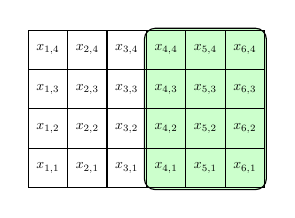
\begin{tikzpicture}[scale=0.5,every node/.style={scale=0.5}]
        % the window
        % offset for x and y of .5 + a bit more (or less)
        \draw[fill=green!20,rounded corners] (3.45,0.45) rectangle (6.55,4.55); % green 
        %% the grid 
        \foreach \l in {1,2,...,4}
        \foreach \c in {1,2,...,6}
        {
          \draw (\c,\l) +(-.5,-.5) rectangle ++(.5,.5);
          \draw (\c,\l) node{$x_{\c,\l}$};
        }
      \end{tikzpicture}
    \end{center}
    %%%%%%%%%%%%%%%%%%%%%%%%%%%%%%
    %%%%%%%%% 2nd column : the questions
    \column{0.66\textwidth}
    The convolution filter generates $h_1$ and $h_2$, and the pooling operation: $o=f(h_1,h_2)$.
    During training the loss gradient should be back-propagated:% through the pooling operation:
      $$
      \frac{\partial \ploss }{\partial \params} = \frac{\partial \ploss }{\partial o} \times \frac{\partial o }{\partial h_i}\times \frac{\partial h_i }{\partial \params}   
      $$
     With mean-pooling:
    \begin{enumerate}
    \item Write $f$ and $\frac{\partial \ploss }{\partial h_i}$ given $\frac{\partial \ploss }{\partial o}$ 
    \item With 2 output channels, at time $1$ $\rightarrow (h_{1,1},h_{1,2})$ and at time $2$ $\rightarrow (h_{2,1},h_{2,2})$, and the pooling $\rightarrow (o_1, o_2)$. Compute the back-prop. gradient. 
    \item For an input of length $L$, how many updates for one filter ? 
    \end{enumerate}
    Reconsider the questions for the max-pooling !
  \end{columns}
\end{frame}

%%%%%%%%%%%%%%%%%%%%%%%%%%%%%%%%%%%%%%%%%%%%%%%%%%%%%%%%%%%%%%%%%%
\begin{frame}{Audio classification / segmentation}
  \framesubtitle{\cite{Jang19Music}}
  \begin{center}
    \includegraphics[width=0.6\textwidth]{../figs/music_speech}    
  \end{center}
  \begin{itemize}
  \item Classification at each time step
  \item But the context is crucial (for the input and the output) ! 
  \item \important{Spectrogram ?}
  \end{itemize}
\end{frame}


%%%%%%%%%%%%%%%%%%%%%%%%%%%%%%%%%%%%%%%%%%%%%%%%%%%%%%%%%%%%%%%%%%
\begin{frame}{Interlude: the input spectrogram}
  \begin{center}
    \includegraphics[width=0.5\textwidth]{../figs/speech_1}\\
    $\downarrow$ \\
    Segmentation in frames (Hamming window)\\
    $\downarrow$ \\
    F.F.T \\
    $\downarrow$ \\
    Mel Filters \\
    $\downarrow$ \\
    Log\\
    $\downarrow$ \\
    D.C.T  \\
    $\downarrow$ \\
    \includegraphics[width=0.5\textwidth]{../figs/speech_2}\\
  \end{center}
\end{frame}



\begin{frame}{Human activity Recognition}
  \begin{block}{The data}
    10k samples of fixed length (128 points at 50kHz)
    \footnote{\url{https://archive.ics.uci.edu/ml/datasets/human+activity+recognition+using+smartphones}}:
    \begin{itemize}
    \item x, y, and z accelerometer data (linear acceleration) 
    \item and the three gyroscopic data (angular velocity)
    \end{itemize}
    The classes are: Walking, Upstairs,  Downstairs,  Sitting,  Standing, Laying. 
  \end{block}
  \begin{itemize}
  \item[$\rightarrow$] Two different input channels (accelerometer and
    gyroscopic).
  \item[$\rightarrow$] How to define a convolution filter for two
    input channels ?
  \item[$\rightarrow$] The sequence is long but of fixed size, the
    overall max-pooling is maybe not the best option.
  \end{itemize}
\end{frame}


\begin{frame}{Convolution 1D with 2 input channels}
    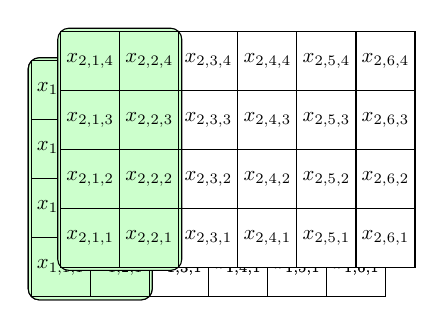
\begin{tikzpicture}[scale=0.75,every node/.style={scale=0.75}]
      % the window 
      % offset for x and y of .5 + a bit more
      %%%% channel 1 
      \draw[fill=green!20,rounded corners] (0.45,0.45) rectangle (2.55,4.55); % green 
      %% the grid 
      \foreach \l in {1,2,...,4}
      \foreach \c in {1,2,...,6}
      {
        \draw (\c,\l) +(-.5,-.5) rectangle ++(.5,.5);
        \draw (\c,\l) node{$x_{1,\c,\l}$};
      }
      %%%% channel 1 
      \draw[fill=green!20,rounded corners] (0.45,0.45) rectangle (2.55,4.55); % green 
      %% the grid 
      \foreach \l in {1,2,...,4}
      \foreach \c in {1,2,...,6}
      {
        \draw (\c,\l) +(-.5,-.5) rectangle ++(.5,.5);
        \draw (\c,\l) node{$x_{1,\c,\l}$};
      }
      %\pause
      %%%% channel 2 
      \draw[fill=white] (1,1) rectangle (7,5);
      \draw[fill=green!20,rounded corners] (0.95,0.95) rectangle (3.05,5.05); % green 
      %% the grid 
      \foreach \l in {1,2,...,4}
      \foreach \c in {1,2,...,6}
      {
        \draw (\c,\l) rectangle ++(1,1);
        \draw (\c,\l)+(0.5,0.5) node{$x_{2,\c,\l}$};
      }
    \end{tikzpicture}
    \hfill
    %\pause
    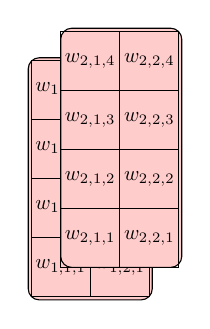
\begin{tikzpicture}[scale=0.75,every node/.style={scale=0.75}]
      %%% channel 1 
      % the window
      % offset for x and y of .5 + a bit more 
      \draw[fill=red!20,rounded corners] (0.45,0.45) rectangle (2.55,4.55); % green 
      %% the grid 
      \foreach \l in {1,2,...,4}
      \foreach \c in {1,2}
      {
        \draw (\c,\l) +(-.5,-.5) rectangle ++(.5,.5);
        \draw (\c,\l) node{$w_{1,\c,\l}$};
      }
      %\pause
      %%% channel 2
      \draw[fill=red!20,rounded corners] (1,1) rectangle (3.05,5.05); % green 
      %% the grid 
      \foreach \l in {1,2,...,4}
      \foreach \c in {1,2}
      {
        \draw (\c,\l) rectangle ++(1,1);
        \draw (\c,\l)+(0.5,0.5) node{$w_{2,\c,\l}$};
      }
    \end{tikzpicture}
    \begin{block}{The output value (output channel)}
      $$
      \textrm{At time }t = 1,\ {\color{red!70!black} h_1} = \sum_{k,i,j} {\color{red!70!black}w_{k,i,j}}\times  {\color{green!70!black}x_{k,i,j}}
      $$
    \end{block}
    We can have multiple input and output channels. 
  \end{frame}



  \begin{frame}{Convolution 1D and max-pooling in pytorch}
    \begin{columns}
      \column{0.5\textwidth}
      \begin{block}{Convolution 1D}
        torch.nn.Conv1d(
        \begin{itemize}
        \item in\_channels, 
        \item out\_channels, 
        \item kernel\_size, 
        \item stride=1, 
        \item padding=0,
        \item dilation=1, ...
        \end{itemize}
        )
      \end{block}
      \column{0.5\textwidth}
      \begin{block}{Max-Pooling 1D}
      torch.nn.MaxPool1d(
      \begin{itemize}
      \item kernel\_size, 
      \item stride=None, 
      \item padding=0, 
      \item dilation=1,
      \item return\_indices=False, 
      \item ceil\_mode=False
      \end{itemize}
      )
    \end{block}
    \end{columns}
  \end{frame}




